% % % 
% % % temp file written by script on Thu Feb 24 16:00:43 2022
% % % lines commented thusly have been or altered by this script
% % % 
\documentclass[border=1pt, 12pt, tikz]{standalone}

\newcommand\wideOne{3cm}
\newcommand\wideTwo{3.5cm}
\newcommand\wideThree{2.7cm}
\newcommand\wideFour{3cm}
\newcommand\distOne{2cm}
\newcommand\distTwo{1cm}

% % % beginning of text inserted by script
% % % 
% % % 
% % % end of text inserted by script
\begin{document}
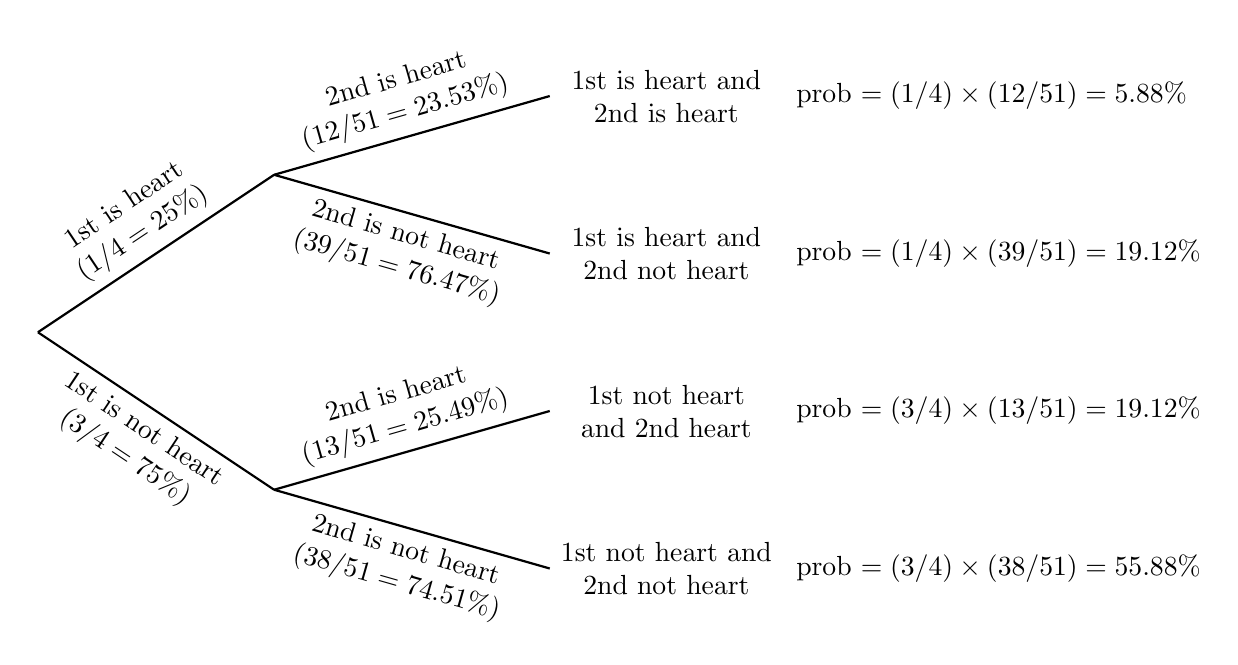
\begin{tikzpicture}[scale=1]

% 1st level
\draw[thick]%
(0,0)
-- node[above, sloped, align=center]
{1st is heart \\ ($1/4=25\%$)}
(\wideOne,\distOne);
\draw[thick]
(0,0)
-- node[below, sloped, align=center]
{1st is not heart\\($3/4=75\%$)}
(\wideOne,-\distOne);

% 2nd, 3rd and 4th Level
\draw[thick]
(\wideOne,\distOne)
-- node[above, align=center, sloped]
{2nd is heart\\ ($12/51=23.53\%$)}
++ (\wideTwo,\distTwo)
node[right, align=center, text width=\wideThree]
{1st is heart and\\2nd is heart}
++ (\wideFour,0)
node[right]
{prob $=(1/4)\times(12/51)=5.88\%$}
;
\draw[thick]
(\wideOne,\distOne)
-- node[below, align=center, sloped]
{2nd is not heart\\ ($39/51=76.47\%$)}
++ (\wideTwo,-\distTwo)
node[right, align=center, text width=\wideThree]
{1st is heart and 2nd not heart}
++ (\wideFour,0)
node[right]
{prob $=(1/4)\times(39/51)=19.12\%$}
;
\draw[thick]
(\wideOne,-\distOne)
-- node[above, align=center, sloped]
{2nd is heart\\ ($13/51=25.49\%$)}
++ (\wideTwo,\distTwo)
node[right, align=center, text width=\wideThree]
{1st not heart and 2nd heart}
++ (\wideFour,0)
node[right]
{prob $=(3/4)\times(13/51)=19.12\%$}
;
\draw[thick]
(\wideOne,-\distOne)
-- node[below, align=center, sloped]
{2nd is not heart\\ ($38/51=74.51\%$)}
++ (\wideTwo,-\distTwo)
node[right, align=center, text width=\wideThree]
{1st not heart and 2nd not heart}
++ (\wideFour,0)
node[right]
{prob $=(3/4)\times(38/51)=55.88\%$}
;
\end{tikzpicture}
\end{document}

% EAJ - attempt with angles follows. But it has horizontal alignment issues.
% \newcommand\angleOne{30}
% \newcommand\angleTwoOut{20}
% \newcommand\angleTwoIn{10}

% \begin{document}
% \begin{tikzpicture}[scale=1.1]

% \draw[thick]%
%    (0:0)
%    -- node[above, pos=0.5, rotate=\angleOne, align=center]{heart \\ ($1/4=25\%$)}
%    (\angleOne:3);
% \draw[thick]
%    (\angleOne:3)
%    -- node[above, align=center, pos=0.5, rotate=\angleTwoOut]{divisible by 3\\ ($1/3=33.33\%$)}
%    ++(\angleTwoOut:3) node[right, align=center, text width=2.6cm]{heart and divisible by 3}
%    ++(0:2.7) node[right]{prob $=(1/4)\times(1/3)=8.33\%$};
% \draw[thick]
%    (\angleOne:3)
%    -- node[below, align=center, pos=0.5, rotate=-\angleTwoIn]{not divisible by 3\\ ($2/3=66.67$)}
%    ++(-\angleTwoIn:3) node[right, align=center, text width=2.6cm]{heart and not divisible by 3}
%    ++(0:2.7) node[right]{prob $=(1/4)\times(2/3)=16.67\%$};

% \draw[thick]
%    (0:0)
%    -- node[below, pos=0.5, rotate=-\angleOne, align=center]{not a heart\\($3/4=75\%$)}
%    (-\angleOne:3);
% \draw[thick]
%    (-\angleOne:3)
%    -- node[above, align=center, pos=0.5, rotate=\angleTwoIn]{divisible by 3\\ ($1/3=33.33\%$)}
%    ++(\angleTwoIn:3) node[right, align=center, text width=2.6cm]{not a heart and divisible by 3}
%    ++(0:2.7) node[right]{prob $=(3/4)\times(1/3)=25\%$};
% \draw[thick]
%    (-\angleOne:3)
%    -- node[below, align=center, pos=0.5, rotate=-\angleTwoOut]{not divisible by 3\\ ($2/3=66.67$)}
%    ++(-\angleTwoOut:3) node[right, align=center, text width=2.6cm]{not a heart and not divisible by 3}
%    ++(0:2.7) node[right]{prob $=(3/4)\times(2/3)=50\%$};
% \end{tikzpicture}
% \end{document}
